\hrefsection{tsfi.ls.lan}{\tsfisectionname{ls.lan}}

\lslan{} ist eine logische Schnittstelle zu den Clientsystemen, die physisch
über das LAN (\intf{PS.LAN}) erreichbar sind.

Die Schnittstelle umfasst die folgenden Protokolle,
\tableref{tab:ls.lan.protocols-ports} listet diese Protokolle und die dafür
verwendeten Portnummern.  \figureref{fig:tsfi.ls.lan.protocols} stellt die
Protokolle dar, welche die sicherheitsrelevanten Aspekte des TSFI ausmachen
(vgl. die einleitende Bemerkung zu \chapterref{tsfi.ls}).

\begin{description}
\item[Ethernet] für Netzzugang,
\item[IP] für Routing,	
\item[TCP und UDP] für die Transportschicht,
\item[DHCP] für IP-Adressvergabe im LAN (Client),
\item[TLS] für die Absicherung der Kommunikation der anderen logischen
  Schnittstellen im LAN.
\item[HTTP\_Mgmt] für den Zugriff auf die Management-Schnittstelle
\end{description}

\tableref{tab:ls.lan.protocols-ports} listet die Protokolle und verwendeten
Ports detailreicher auf. Abbildung~\vref{fig:tsfi.ls.lan.protocols} zeigt die
Protokolle der Schnittstelle \lslan{} in Relation zueinander und bezogen auf das
TCP/IP Schichtenmodell. Der Protokollstapel ist aus Platzgründen auf zwei
Abbildungen aufgeteilt.

\afterpage{%
  \clearpage% Flush earlier floats (otherwise order might not be correct)
  \begin{landscape}% Landscape page
    \centering % Center table
    {
      \label{tab:ls.lan.protocols-ports}
\begin{longtable}{@{}lcllcclp{6cm}@{}}
  \toprule
  Service & In/Out & Protocol & via & Source port & Dest. port & TSFI & Note \\ \midrule \endhead
  \bottomrule \caption*{Protocols und port numbers for IP/TCP/UDP on \formatintf{LS.LAN}} \endfoot
  \bottomrule \caption{Protocols und port numbers for IP/TCP/UDP on \formatintf{LS.LAN}} \endlastfoot
  Base protocols & -- & IEEE802.3 &  -- & -- & -- &    \tsfilink{ls.lan.ether} \\
  & -- & IPv4 & IEEE802.3 & -- & -- &    \tsfilink{ls.lan.ip} \\
  & -- & TCP &  IPv4 & -- & -- &    \tsfilink{ls.lan.tcp} \\
  & -- & UDP &  IPv4 & -- & -- &    \tsfilink{ls.lan.udp} \\[2ex]
  Administration & In & TLS & TCP & any & 9443 & \tsfilink{ls.lan.tls} & \\ 
  & In & HTTP & TLS & any & 9443 &  \tsfilink{ls.lan.httpmgmt} \\[2ex]
\end{longtable}


%

%!TEX root = "../adv_fsp"
%%% Local Variables:
%%% mode: latex
%%% TeX-engine: luatex
%%% TeX-master: "../adv_fsp"
%%% TeX-parse-self: t
%%% TeX-auto-save: t
%%% End:

    }
  \end{landscape}
  \clearpage% Flush page
}

\begin{figure}[htbp]
  \centering
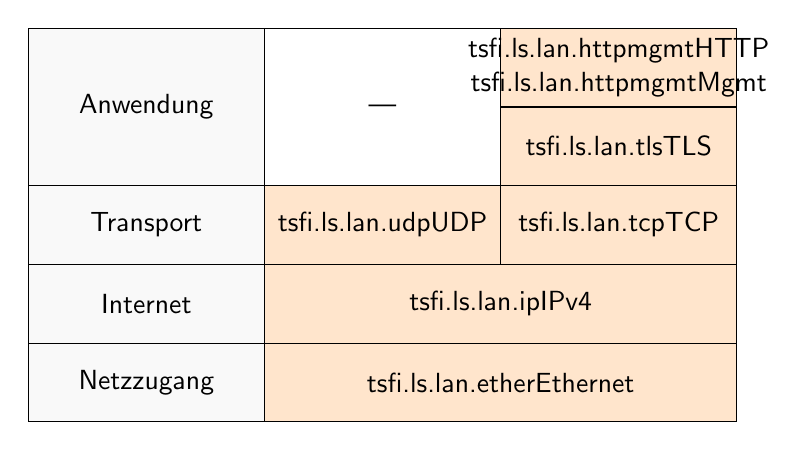
\begin{tikzpicture}
    [c/.style={midway,align=center,font=\sffamily},
      tsfi/.style={fill=orange!20},
      nontsfi/.style={fill=yellow!20},
      none/.style={},
      layer/.style={fill=gray!5}]


  % App Layer für UDP
  \draw[layer] (0,3) rectangle ++(3,2) node[c]{Anwendung};
  \draw[none] (3,3) rectangle ++(3,2) node[c]{---};
  \draw[tsfi] (6,3) rectangle ++(3,1) node[c]{\hyperlink{tsfi.ls.lan.tls}{TLS}};

  \draw[tsfi] (6,4) rectangle ++(3,1) node[c]{\hyperlink{tsfi.ls.lan.httpmgmt}%
    {HTTP}\\\hyperlink{tsfi.ls.lan.httpmgmt}{Mgmt}};

  % Transport Layer
  \draw[layer] (0,2) rectangle ++(3,1) node[c]{Transport};
  \draw[tsfi] (3,2) rectangle ++(3,1) node[c]{\hyperlink{tsfi.ls.lan.udp}{UDP}};
  \draw[tsfi] (6,2) rectangle ++(3,1) node[c]{\hyperlink{tsfi.ls.lan.tcp}{TCP}};

  % IP Layer
  \draw[layer] (0,1) rectangle ++(3,1) node[c]{Internet};
  \draw[tsfi] (3,1) rectangle ++(6,1) node[c]{\hyperlink{tsfi.ls.lan.ip}{IPv4}};

  % Network Layer
  \draw[layer] (0,0) rectangle ++(3,1) node[c]{Netzzugang};
  \draw[tsfi] (3,0) rectangle ++(6,1) node[c]{\hyperlink{tsfi.ls.lan.ether}{Ethernet}};

\end{tikzpicture}
  \caption{Protokolle auf \formatintf{LS.LAN} für die sicherheitsfunktionalen Anteile}
  \label{fig:tsfi.ls.lan.protocols}
\end{figure}

\clearpage

\hrefsubsection{tsfi.ls.lan.ether}{\tsfisectionname{ls.lan.ether}}

\tsfipurpose{tsfi.ls.lan.ether}

Diese Schnittstelle dient als \emph{Netzzugangsschicht} zum
Ethernet-Netzwerk.

\aufgerufenesf{ls.lan.ether}

\tsfiparameters{tsfi.ls.lan.ether}

Die Schnittstelle implementiert das Ethernet-Protokoll nach
\autocite{IEEE802.3}. 

\hrefsubsection{tsfi.ls.lan.ip}{\tsfisectionname{ls.lan.ip}}

\tsfipurpose{tsfi.ls.lan.ip}

Auf der \emph{Internetschicht} verhält sich der TOE als IP-Router und
unterstützt das Internet-Protokoll in der Version 4. Zusätzlich wird das
ICMP-Protokoll unterstützt, welches Teil von IPv4 ist.  

\aufgerufenesf{ls.lan.ip}

\tsfiparameters{tsfi.ls.lan.ip}

Die Implementierung von IPv4 entspricht den Vorgaben aus \rfc[c]{791},
\rfc[c]{1812} und den Aktualisierungen in \rfc[c]{2644}. ICMP ist in
\rfc[c]{792} spezifiziert. Die Implementierung von IPv4 wird durch den
Linux-Kernel bereitgestellt.

\hrefsubsection{tsfi.ls.lan.tcp}{\tsfisectionname{ls.lan.tcp}}

\tsfipurpose{tsfi.ls.lan.tcp}

Auf der \emph{Transportschicht} unterstützt der TOE das Transmission
Control Protocol (TCP). 

\aufgerufenesf{ls.lan.tcp}

\tsfiparameters{tsfi.ls.lan.tcp}

Die Implementierung von TCP entspricht den Vorgaben aus
\rfc[c]{793}. Die Implementierung von TCP wird durch den Linux-Kernel
bereitgestellt.


\hrefsubsection{tsfi.ls.lan.udp}{\tsfisectionname{ls.lan.udp}}

\tsfipurpose{tsfi.ls.lan.udp}

Der TOE unterstützt auf der \emph{Transportschicht} zusätzlich das
User Datagram Protocol (UDP). 

\aufgerufenesf{ls.lan.udp}

\tsfiparameters{tsfi.ls.lan.udp}

Die Implementierung von UDP entspricht den Vorgaben aus
\rfc[c]{768}. Die Implementierung von UDP wird durch den Linux-Kernel
bereitgestellt.

\hrefsubsection{tsfi.ls.lan.tls}{\tsfisectionname{ls.lan.tls}}

\tsfipurpose{tsfi.ls.lan.tls}

\lslantls{} wird verwendet, um Verbindungen zu anderen Systemen im LAN
abzusichern. TLS stellt Vertraulichkeit und
Integrität der Verbindungen sicher. Eine Übersicht über die TLS
Verbindungen und deren Konfiguration des TOE ist in Tabelle
\tableref{tab:tlsconnections} zu finden. 

\aufgerufenesf{ls.lan.tls}

\tsfiparameters{tsfi.ls.lan.tls}

Die Implementierung von TLS im TOE setzt \autocite{rfc5246} um. Die Beschreibung
der TLS-Implementierung sowie allen TLS-Verbindungen des TOE gemeinsamen
Parameter und TOE-spezifische Anpassungen der TLS-Implementierung sind in
Kapitel \ref{sf.tls} dokumentiert.

\hrefsubsection{tsfi.ls.lan.httpmgmt}{\tsfisectionname{ls.lan.httpmgmt}}

\tsfipurpose{tsfi.ls.lan.httpmgmt}

Der TOE implementiert einen HTTP-Server, um die Konfiguration des TOE über die
JSON-Schnittstelle der Webanwendung zu ermöglichen. Die Benutzung der
Webanwendung wird im Administratorhandbuch beschrieben, das als Dokumenttyp
AGD\_ADM ebenfalls Teil der Sicherheitsdokumentation ist \autocite{agd_adm}. Der
TOE liefert an der Schnittstelle \lslanhttpmgmt{} den Code der Webanwendung an
den Web-Browser des Administrators aus. Der Browser interpretiert den Code und
führt ihn aus. Der im Browser ablaufende Code interagiert mit der JSON-API. Die
Frontend-Elemente der Webanwendung (also die HTML-, CSS- und
JavaScript-Elemente) selbst werden nicht näher beschrieben. Sie setzen keine
Sicherheitsanforderungen um. Der Grund dafür ist, dass dieses Frontend auf einem
Browser des Anwenders, also in der Umgebung des TOE, ausgeführt wird und zur
Laufzeit nicht unter der Kontrolle der TSF steht. Der Nutzer hat volle Kontrolle
über die Ausführungsplattform des Frontends und kann beliebig in den dort
ablaufenden JavaScript Code eingreifen. Die Sicherheitsanforderungen der
Managementschnittstelle werden folglich ausschließlich von den serverseitigen
Komponenten erbracht.

Das Protokoll zur Übertragung von Konfigurationsparametern ist in Form einer
JSON-API implementiert. Die serverseitigen Komponenten der Webanwendung nehmen
die fachlichen Werte als API-Aufrufe entgegen. Darüber hinaus sorgen sie für die
Authentisierung des Administrators und den Schutz vor XSS- und
CSRF-Angriffen. Die konkrete Ausgestaltung dieser Schutzmaßnahmen wird in der
Sicherheitsarchitektur beschrieben
\autocite{adv_arc}. Die Prüfung des Authentisierungsstatus
erfolgt fortlaufend, also bei jedem Request.


\aufgerufenesf{ls.lan.httpmgmt}

\tsfiparameters{tsfi.ls.lan.httpmgmt}

Der HTTP-Server implementiert \rfc[c]{2616}. Die Verbindung ist über TLS
abgesichert, vgl. die Beschreibung zu \lslantls{} und
Abschnitt~\ref{sf.tls}.

Die Konfigurationswerte werden als JSON-Objekte an die Schnittstelle
übergeben. Das Transportprotokoll ist HTTP, wobei die Schnittstelle als REST API
zu verwenden ist. Es wird streng unterschieden zwischen Requests, mit denen
statische Elemente angefordert werden, und solchen, die zu schützende Daten wie
Session-IDs oder Benutzerdaten enthalten. Letztere werden ausschließlich über
POST-Requests angefordert, sodass keine zu schützenden Elemente in der
Browser-Historie verbleiben. Die Parameter und die Verwendung der Schnittstelle
werden separat in einer separaten Dokumentation beschrieben. JSON wird in
\rfc[c]{7159} definiert.


% !TEX root = "../adv_fsp"
%%% Local Variables:
%%% mode: latex
%%% TeX-engine: luatex
%%% TeX-master: "../adv_fsp"
%%% TeX-parse-self: t
%%% TeX-auto-save: t
%%% End:
